% This is the HU Berlin LaTeX template, optimized for R Markdown.

% -------------------------------
% --- PREAMBLE ---
% -------------------------------
\documentclass[a4paper,11pt]{article}

\usepackage{amsmath,amssymb,amsfonts,amsthm}    % Typical maths resource packages
\usepackage{graphicx}                           % Packages to allow inclusion of graphics
\usepackage[authoryear]{natbib}                 % literature reference style


\usepackage[bf]{caption}
\usepackage{textcomp}                           % For single quotes
\usepackage{floatrow}                           % For image and table position
\usepackage{booktabs}                           % For tables
% \usepackage[colorlinks=true]{hyperref}                           
% \usepackage[bottom]{footmisc}                   
\usepackage[bottom, flushmargin]{footmisc}                   % For footnotes
\usepackage[citebordercolor={0 1 0}]{hyperref}                           % For creating hyperlinks in cross references
\usepackage{footnotebackref}

% -------------------------------
% --- some layout definitions ---
% -------------------------------

% define topline
\usepackage[automark]{scrlayer-scrpage}
\pagestyle{scrheadings}
\automark{section}
\clearscrheadings
\ohead{\headmark}

% define citation style
\bibliographystyle{ecta}

% define page size, margin size
\setlength{\headheight}{1.1\baselineskip}
\voffset=-2cm
\hoffset=-3cm
\textheight24cm
\textwidth15.5cm
\topmargin1cm
\oddsidemargin3cm
\evensidemargin3cm
\setcounter{secnumdepth}{3}
\setcounter{tocdepth}{3}   
  \usepackage[parfill]{parskip} 

% define line spacing = 1.5
\renewcommand{\baselinestretch}{1.5}

% define position of graphics
\floatsetup[figure]{capposition=bottom}
\floatsetup[table]{capposition=bottom}
\floatplacement{figure}{ht}
\floatplacement{table}{ht}

% save thesis parameters for later
\newcommand{\thesistype}{Master's Thesis}
\newcommand{\thesisauthor}{Harm van Kuppevelt}
\newcommand{\thesisdate}{June, 2021}

% define tightlist to work with newer versions of pandoc
\providecommand{\tightlist}{%
  \setlength{\itemsep}{0pt}\setlength{\parskip}{0pt}}


\newlength{\cslhangindent}
\setlength{\cslhangindent}{1.5em}
\newenvironment{CSLReferences}%
  {}%
  {\par}

% change spacing
\setlength {\parskip}{1em}

% Additional LaTeX parameters added in the YAML header of index.Rmd



% --------------------------------------
% --------------------------------------
% --------------------------------------
% --- the structure the tex document ---
% ---  (this our recommendation) -------
% frontmatter:
%   - titlepage (mandatory),
%   - acknowledgement,
%   - abstract,
%   - table of contents (mandatory),
%   - list of abbreviations (not mandatory),
%   - list of figures (not mandatory),
%   - list of tables  (not mandatory) .
%
% body of the thesis (the structure of the thesis body is not mandatory, but the list of literature is mandatory):
%   - introduction,
%   - methods,
%   - data,
%   - results,
%   - conclusion,
%   - literature (mandatory),
%   - appendix (figures, tables).
%
% last page:
%   - declaration of authorship (mandatory).
% --------------------------------------
% --------------------------------------
% --------------------------------------
\begin{document}
% -------------------------------
% --- frontmatter: Title page ---
% -------------------------------
\thispagestyle{empty}
\begin{center}
  {\Large{\bf Phosphate dynamics in iron treated peat ditches}} \vspace{0.5cm}

  Master's Thesis submitted \\\vspace{0.5cm}
  to \\\vspace{0.5cm}
  \textbf{Dr.~Thilo Behrends} \\
  \textbf{Melanie Münch Msc.} \\\vspace{0.5cm}
  Utrecht University \\
  Faculty of Geosciences \\
  Department of Earth sciences \\
   Geochemistry \\  \vspace{1cm}

  
\includegraphics[width=0.5\textwidth]{UU_logo_EN_CMYK.png}
  
  by \\\vspace{0.5cm}
  \textbf{Harm van Kuppevelt} \\
  (4061985) \\
  
  \medskip
  \medskip
  in partial fulfillment of the requirements \\
  for the degree of \\
  \textbf{Master of Earth Science} \\\vspace{0.5cm}
  June, 2021
  
\end{center}
% ------------------------------------
% --- frontmatter: Acknowledgement ---
% ------------------------------------
\newpage
\hypertarget{acknowledgements}{%
\section*{Acknowledgements}\label{acknowledgements}}
\addcontentsline{toc}{section}{Acknowledgements}

I want to thank food for existing.
\pagestyle{plain}
\pagenumbering{roman}   % define page number in roman style
\setcounter{page}{1}    % start page numbering

% -----------------------------
% --- frontmatter: Abstract ---
% -----------------------------
\newpage
\hypertarget{abstract}{%
\section*{Abstract}\label{abstract}}
\addcontentsline{toc}{section}{Abstract}

Lorem ipsum dolor sit amet, consectetur adipiscing elit, sed do eiusmod tempor incididunt ut labore et dolore magna aliqua. Ut enim ad minim veniam, quis nostrud exercitation ullamco laboris nisi ut aliquip ex ea commodo consequat. Duis aute irure dolor in reprehenderit in voluptate velit esse cillum dolore eu fugiat nulla pariatur. Excepteur sint occaecat cupidatat non proident, sunt in culpa qui officia deserunt mollit anim id est laborum.

% -----------------------------
% --- frontmatter: Contents ---
% -----------------------------
\newpage
\tableofcontents
\clearpage

% ----------------------------------------------------------
% --- frontmatter: List of Abbreviations (not mandatory) ---
% ----------------------------------------------------------

% ----------------------------------------------------
% --- frontmatter: List of Figures (not mandatory) ---
% ----------------------------------------------------
\newpage
\listoffigures
\addcontentsline{toc}{section}{List of Figures}

% ---------------------------------------------------
% --- frontmatter: List of Tables (not mandatory) ---
% ---------------------------------------------------
\newpage
\listoftables
\addcontentsline{toc}{section}{List of Tables}

% -------------------------------
% --- main body of the thesis ---
% -------------------------------
\newpage
\pagestyle{plain}       
\setcounter{page}{1}    % start page numbering anew
\pagenumbering{arabic}  % page numbers in arabic style

\hypertarget{preface}{%
\section*{Preface}\label{preface}}
\addcontentsline{toc}{section}{Preface}

Welcome to the thesis template. This template is based on (and in many places
copied directly from) the HU Berlin School of Business and Economics LaTeX
template, but hopefully it will provide a nicer interface for those that have
never used LaTeX before.

\hypertarget{introduction}{%
\section{Introduction}\label{introduction}}
\begin{itemize}
\item
  What is the subject of the study? Describe the problem.
\item
  What is the purpose of the study (working hypothesis)?
\item
  What do we already know about the subject (literature review)? Use citations:
  \protect\hyperlink{ref-lingenfelser2011systematic}{Lingenfelser, Wagner, and André} (\protect\hyperlink{ref-lingenfelser2011systematic}{2011}) shows that\ldots{} Alternative Forms of the Wald test are
  considered (\protect\hyperlink{ref-kuncheva2004combining}{Kuncheva 2004}).
\item
  What is the innovation of the study?
\item
  Provide an overview of your results.
\item
  Outline of the paper:\\
  \emph{The paper is organized as follows. The next section describes the model
  under investigation. Section ``{[}Data{]}'' describes the data set
  and Section ``\protect\hyperlink{results}{Results}'' presents the results. Finally, Section
  ``\protect\hyperlink{conclusion}{Conclusion}'' concludes.}
\item
  The introduction should not be longer than 4 pages.
\end{itemize}
\hypertarget{methodology}{%
\section{Methodology}\label{methodology}}

\hypertarget{results}{%
\section{Results}\label{results}}
\begin{verbatim}
[1] "C:/Users/harmv/Documents/studie/scriptie/Master/Master_Thesis/index"
\end{verbatim}
\begin{verbatim}
here() starts at C:/Users/harmv/Documents/studie/scriptie/Master/Master_Thesis
\end{verbatim}
\begin{verbatim}
-- Attaching packages --------------------------------------- tidyverse 1.3.1 --
\end{verbatim}
\begin{verbatim}
v tibble  3.1.2     v purrr   0.3.4
v tidyr   1.1.3     v stringr 1.4.0
v readr   1.4.0     v forcats 0.5.1
\end{verbatim}
\begin{verbatim}
-- Conflicts ------------------------------------------ tidyverse_conflicts() --
x dplyr::filter()          masks stats::filter()
x kableExtra::group_rows() masks dplyr::group_rows()
x dplyr::lag()             masks stats::lag()
\end{verbatim}
\begin{center}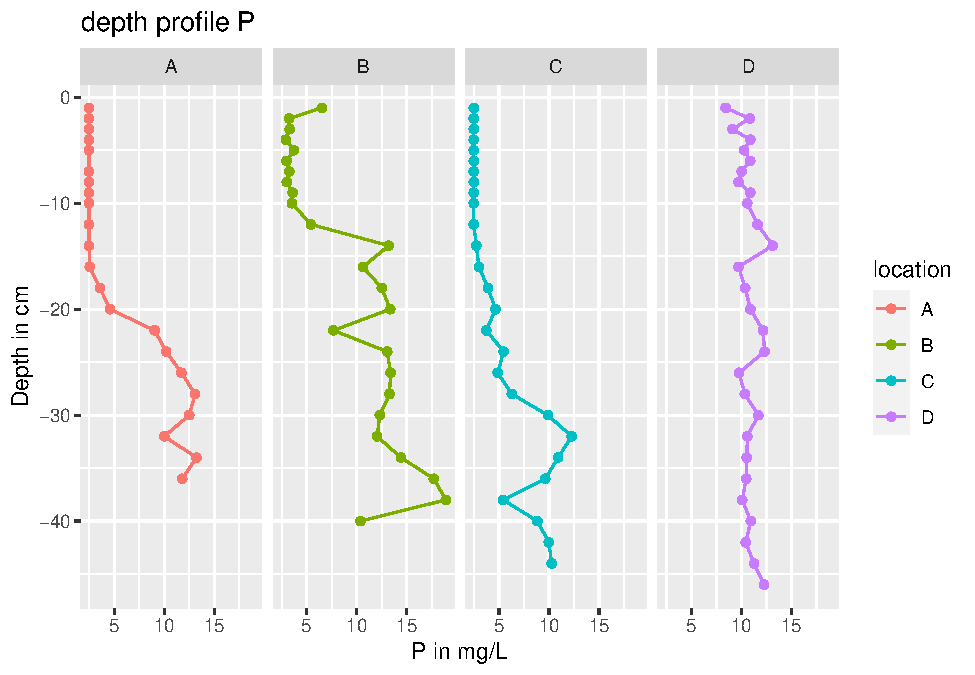
\includegraphics{thesis_files/figure-latex/ICgraphs-1} \end{center}
\begin{center}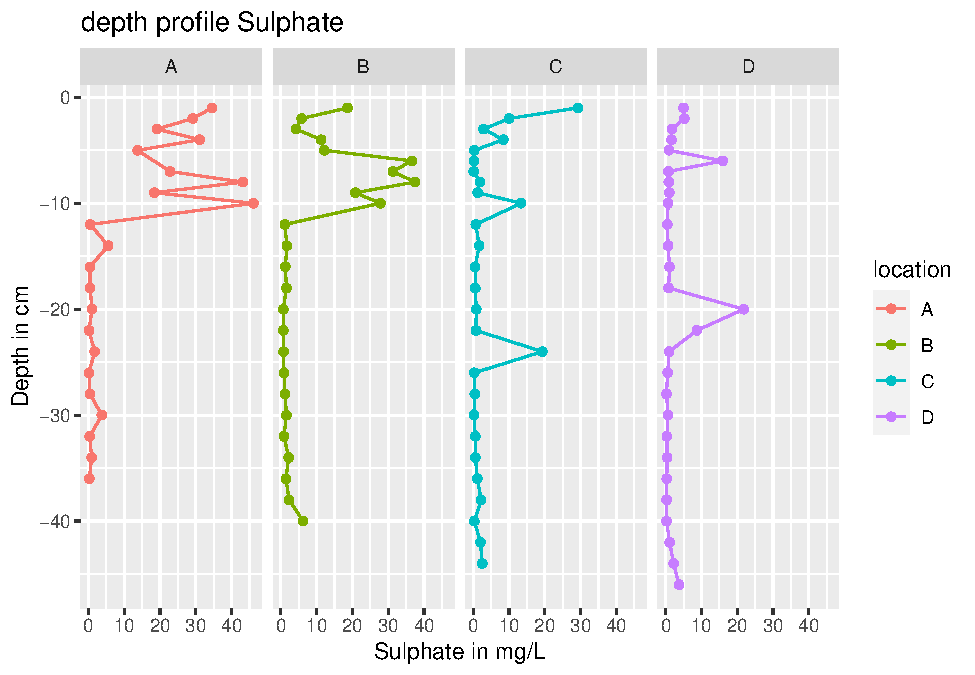
\includegraphics{thesis_files/figure-latex/ICgraphs-2} \end{center}
\begin{center}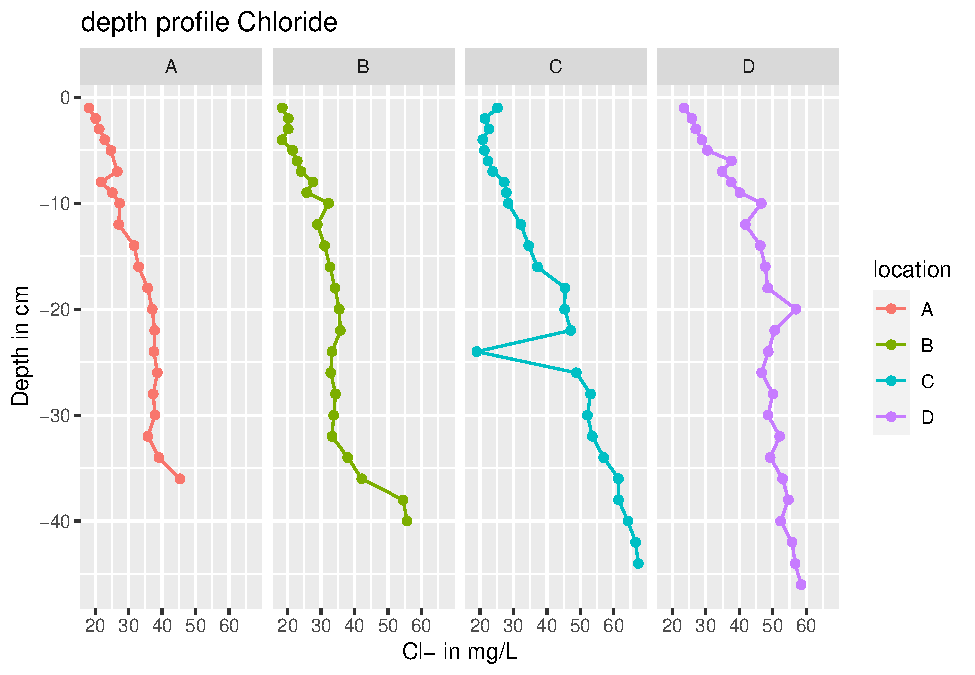
\includegraphics{thesis_files/figure-latex/ICgraphs-3} \end{center}
\begin{center}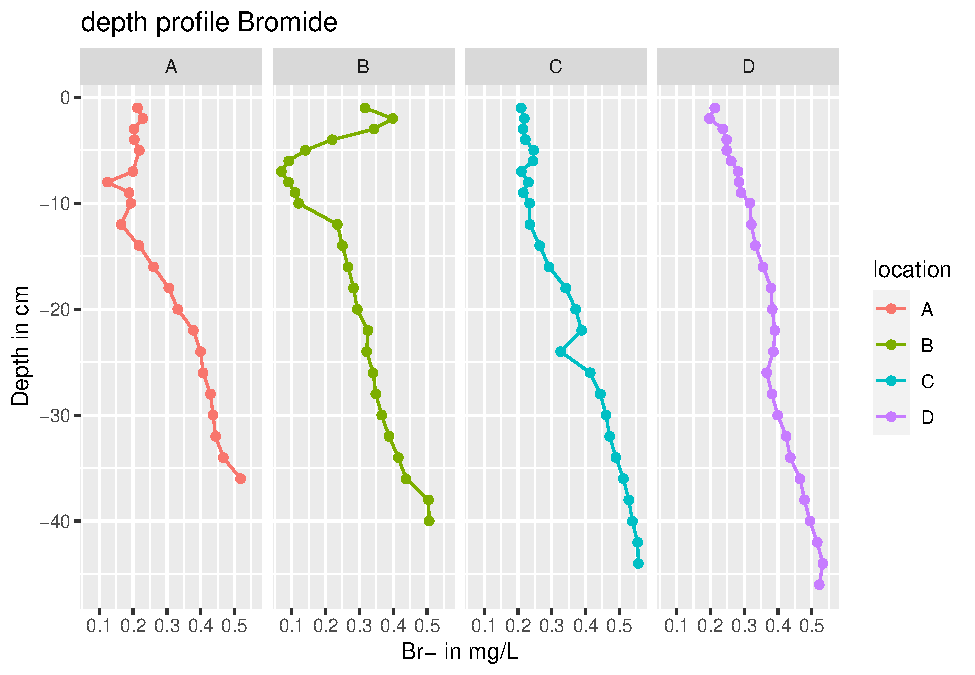
\includegraphics{thesis_files/figure-latex/ICgraphs-4} \end{center}
\begin{center}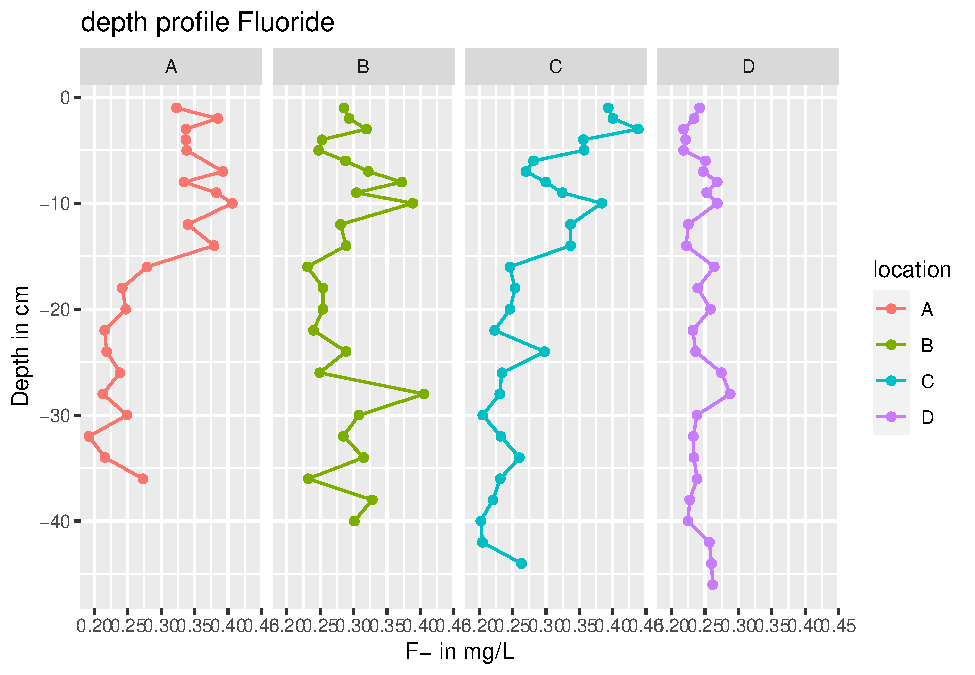
\includegraphics{thesis_files/figure-latex/ICgraphs-5} \end{center}
\begin{itemize}
\item
  Organize material and present results.
\item
  Use tables, figures (but prefer visual presentation):
  \begin{itemize}
  \item
    Tables and figures should supplement (and not duplicate) the text.
  \item
    Tables and figures should be provided with legends.
  \item
    \emph{Figure \ref{fig:graph} shows how to include and reference graphics.
    The graphic must be labelled before. Files must be in \textbf{.eps} format. You
    can do this really easily in R Markdown with \texttt{knitr::include\_graphics()}}!
  \item
    Figures can be referenced with \texttt{\textbackslash{}@ref(fig:\textless{}name\textgreater{})}, where \texttt{\textless{}name\textgreater{}} is the
    name of the code chunk.
  \end{itemize}
\end{itemize}
\begin{figure}

{\centering \includegraphics[width=0.5\linewidth]{C:/Users/harmv/Documents/studie/scriptie/Master/Master_Thesis/index/figures/graph} 

}

\caption{Estimated residuals from model XXX. ...}\label{fig:graph}
\end{figure}
\begin{itemize}
\tightlist
\item
  Tables and graphics may appear in the text or in the appendix, especially if
  there are many simulation results tabulated, but is also depends on the study
  and number of tables resp. figures. The key graphs and tables must appear in
  the text!
\end{itemize}
\begin{table}[H]

\caption{\label{tab:table}Detailed descriptive statistics of location and dispersion for 2100 observed swap rates for the period from February 15, 1999 to March 2, 2007. Swap rates measured as 3.12 (instead of 0.0312).}
\centering
\begin{tabular}[t]{lrrrrrrrrrr}
\toprule
  & 3m & 6m & 1yr & 2yr & 3yr & 5yr & 7yr & 10yr & 12yr & 15yr\\
\midrule
Mean & 3.138 & 3.191 & 3.307 & 3.544 & 3.756 & 4.093 & 4.354 & 4.621 & 4.741 & 4.878\\
StD & 0.915 & 0.919 & 0.935 & 0.910 & 0.876 & 0.825 & 0.803 & 0.776 & 0.768 & 0.762\\
\midrule
\bottomrule
\end{tabular}
\end{table}
\begin{itemize}
\item
  Allows the reader to judge whether the sample is biased or to evaluate
  possible impacts of outliers, for example.
\item
  Here tables can be easily integrated using the \texttt{kable()} function in the
  \texttt{knitr} package (with perhaps some additional help from the \texttt{kableExtra}
  package). \texttt{kable()} will automatically generate a label for the table
  environment. That way you don't have to manually enter in the table in LaTex,
  you can embed tables from R code.
\item
  Tables can be referenced using \texttt{\textbackslash{}@ref(label)}, where \texttt{label} is \texttt{tab:\textless{}name\textgreater{}},
  where \texttt{\textless{}name\textgreater{}} is the code chunk label.
\item
  The appearance may look different to tables directly typed with LaTex, due to
  limitations in \texttt{kable()}. To compare:
  \begin{table}[ht]
    \begin{center}
        {\footnotesize
        \begin{tabular}{l|cccccccccc}
            \hline \hline
                      & 3m    & 6m    & 1yr   & 2yr   & 3yr   & 5yr   & 7yr   & 10yr  & 12yr  & 15yr   \\
            \hline
                Mean   & 3.138 & 3.191 & 3.307 & 3.544 & 3.756 & 4.093 & 4.354 & 4.621 & 4.741 & 4.878  \\
                StD    & 0.915 & 0.919 & 0.935 & 0.910 & 0.876 & 0.825 & 0.803 & 0.776 & 0.768 & 0.762  \\
            \hline \hline
        \end{tabular}}
    \end{center}
    \caption{This table was handwritten with LaTeX.}
    \label{tab:table2}
    \end{table}
\item
  R Markdown can also supports math equations just like \emph{LaTeX}!
  \begin{itemize}
  \item
    \emph{Equation \eqref{eq:SpecDens} represents the ACs of a stationary
    stochastic process:}
    \begin{equation}
            f_y(\lambda) = (2\pi)^{-1} \sum_{j=-\infty}^{\infty}
                           \gamma_j e^{-i\lambda j}
                         =(2\pi)^{-1}\left(\gamma_0 + 2 \sum_{j=1}^{\infty}
        \gamma_j \cos(\lambda j)\right)
                                       \label{eq:SpecDens}
    \end{equation}
    \emph{where \(i=\sqrt{-1}\) is the imaginary unit, \(\lambda \in [-\pi, \pi]\) is the
    frequency and the \(\gamma_j\) are the autocovariances of \(y_t\).}
  \item
    Equations can be referenced with \texttt{\textbackslash{}@ref(eq:\textless{}name\textgreater{})}, where name is defined
    by adding \texttt{(\textbackslash{}\#eq:\textless{}name\textgreater{})} in the line immediately before \texttt{\textbackslash{}end\{equation\}}.
  \end{itemize}
\end{itemize}
\hypertarget{review-of-results}{%
\subsection{Review of Results}\label{review-of-results}}
\begin{itemize}
\item
  Do the results support or do they contradict theory ?
\item
  What does the reader learn from the results?
\item
  Try to give an intuition for your results.
\item
  Provide robustness checks.
\item
  Compare to previous research.
\end{itemize}
\hypertarget{discussion}{%
\section{Discussion}\label{discussion}}

\hypertarget{conclusion}{%
\section{Conclusion}\label{conclusion}}
\begin{itemize}
\item
  Give a short summary of what has been done and what has been found.
\item
  Expose results concisely.
\item
  Draw conclusions about the problem studied. What are the implications of your
  findings?
\item
  Point out some limitations of study (assist reader in judging validity of
  findings).
\item
  Suggest issues for future research.
\end{itemize}
\newpage

\hypertarget{references}{%
\section*{References}\label{references}}
\addcontentsline{toc}{section}{References}

\noindent

\setlength{\parindent}{-0.5cm}
\setlength{\leftskip}{0.5cm}
\setlength{\parskip}{8pt}

\hypertarget{refs}{}
\begin{CSLReferences}{1}{0}
\leavevmode\hypertarget{ref-kuncheva2004combining}{}%
Kuncheva, Ludmila I. 2004. \emph{Combining Pattern Classifiers: Methods and Algorithms}. John Wiley \& Sons.

\leavevmode\hypertarget{ref-lingenfelser2011systematic}{}%
Lingenfelser, Florian, Johannes Wagner, and Elisabeth André. 2011. {``A Systematic Discussion of Fusion Techniques for Multi-Modal Affect Recognition Tasks.''} In \emph{Proceedings of the 13th International Conference on Multimodal Interfaces}, 19--26. ACM.

\end{CSLReferences}
\indent
\setlength{\parindent}{17pt}
\setlength{\leftskip}{0pt}
\setlength{\parskip}{0pt}

\newpage

\appendix

\hypertarget{appendix}{%
\section{Appendix}\label{appendix}}

Here goes the appendix!

\hypertarget{figures}{%
\subsection{Figures}\label{figures}}
\begin{figure}

{\centering \includegraphics[width=0.5\linewidth,]{figures/graph} 

}

\caption{Estimated residuals (2) from model XXX. ...}\label{fig:graph2}
\end{figure}
\hypertarget{tables}{%
\subsection{Tables}\label{tables}}
\begin{table}[ht]
    \begin{center}
        {\footnotesize
        \begin{tabular}{l|cccccccccc}
        \hline \hline
                        & 3m    & 6m    & 1yr   & 2yr   & 3yr   & 5yr   & 7yr   & 10yr  & 12yr  & 15yr   \\
            \hline
                Mean   & 3.138 & 3.191 & 3.307 & 3.544 & 3.756 & 4.093 & 4.354 & 4.621 & 4.741 & 4.878  \\
                Median & 3.013 & 3.109 & 3.228 & 3.490 & 3.680 & 3.906 & 4.117 & 4.420 & 4.575 & 4.759  \\
                Min    & 1.984 & 1.950 & 1.956 & 2.010 & 2.240 & 2.615 & 2.850 & 3.120 & 3.250 & 3.395  \\
                Max    & 5.211 & 5.274 & 5.415 & 5.583 & 5.698 & 5.805 & 5.900 & 6.031 & 6.150 & 6.295  \\
                StD    & 0.915 & 0.919 & 0.935 & 0.910 & 0.876 & 0.825 & 0.803 & 0.776 & 0.768 & 0.762  \\
            \hline \hline
        \end{tabular}}
    \end{center}
    \caption{Detailed descriptive statistics of location and dispersion for
    2100 observed swap rates for the period from
    February 15, 1999 to March 2, 2007. Swap rates measured as 3.12 (instead of 0.0312).}
    \label{tab:apptable}
\end{table}
\newpage

% change rmd_files in `_bookdown.yml` files to determine order
% note that references and appendix are also contained here.


% --------------------------------------------
% --- last page: Declaration of Authorship ---
% --------------------------------------------

\newpage
\thispagestyle{empty}
\hypertarget{declaration-of-authorship}{%
\section*{Declaration of Authorship}\label{declaration-of-authorship}}

I hereby confirm that I have authored this \thesistype{} independently and
without use of others than the indicated sources. All passages which are
literally or in general matter taken out of publications or other sources are
marked as such.
\vspace{1cm}

Berlin, \thesisdate{}
\vspace{3cm}

. . . . . . . . . . . . . . . . . . . . . . . . . . . . . . .
\vspace{0.1cm}

\thesisauthor{}


\end{document}
